\documentclass[11pt,a4paper, halfparskip]{scrartcl}
\usepackage[utf8]{inputenc}
\usepackage[ngerman]{babel}
\usepackage[T1]{fontenc}
\usepackage{amsmath}
\usepackage{amsfonts}
\usepackage{amssymb}
\usepackage{graphicx}
\usepackage[bookmarksnumbered,pdftitle={Name}]{hyperref}
\usepackage[left=2cm,right=2cm,top=2cm,bottom=2cm]{geometry}
\usepackage{lmodern}
\usepackage{listings}
\usepackage{xcolor}
\usepackage{tabularx}

\usepackage{geometry}
\geometry{a4paper, top=25mm, left=40mm, right=40mm, bottom=30mm,
headsep=10mm, footskip=12mm}

\title{Bericht zum Laborprojekt}
\author{Ali Al-Ali \and Jonathan Lange \and Jeremy Puchta \and }
\renewcommand*{\titlepagestyle}{empty}

\definecolor{background}{HTML}{FFFFFF}

\lstdefinelanguage{json} {
    basicstyle=\normalfont\ttfamily,
    numbers=left,
    numberstyle=\scriptsize,
    stepnumber=1,
    numbersep=8pt,
    showstringspaces=false,
    breaklines=true,
    frame=lines,
    backgroundcolor=\color{background},
}

\begin{document}

\begin{titlepage}
	\centering
	
\includegraphics[width=1\textwidth]{Unilogo}\par\vspace{1cm}
	{\scshape\LARGE Universität Leipzig \par}
	\vspace{0.5cm}
	{\scshape\Large Abteilung Automatische Sprachverarbeitung\par}
	\vspace{0.2cm}
	{\scshape\large Fortgeschrittene Methoden des Information Retrieval\par}
	\vspace{1cm}
	{\huge\bfseries Bericht zum Laborprojekt\par}
	\vspace{1cm}
	{\Large Ali Al-Ali -- Jonathan Lange -- Jeremy Puchta \par}

	\vfill
	
	{\large \today\par}
\end{titlepage}

\newpage

\thispagestyle{empty}
\tableofcontents

\newpage
\pagenumbering{arabic}
\section{Einleitung}

Der vorliegende Bericht erläutert den Aufbau sowie die Funktionsweise der Suchmaschine \textit{Historical News Search}, welche im Rahmen des Laborprojektes innerhalb des Moduls \textit{Fortgeschrittene Methoden des Information Retrieval} im Wintersemester 2018 / 2019 erstellt wurde. 
Ziel des Laborprojektes war es, die vermittelten Vorlesungsinhalte zu vertiefen und diese bei der Erstellung einer domänenspezifischen Suchmaschine umzusetzen. 
Die vorgestellte Suchmaschine dient der Exploration von historischen Nachrichten und Zeitungsartikeln.
Als Anwendungsfälle für eine solche Suchmaschine sind verschiedene Szenarien denkbar. 
Ein Nutzer kann beispielsweise nach der Berichterstattung zu Personen, Gruppen, Orten oder bestimmten historischen Ereignissen suchen.
Eine weitere Möglichkeit der Nutzung stellt die Ahnenforschung dar, bei welcher ein Nutzer in Zeitungsberichten nach Informationen über seine Vorfahren suchen und somit mehr über seine Familienhistorie erfahren kann.

Im folgenden Kapitel wird zunächst der verwendete Technologiestack eingehend beschrieben.
Anschließend erfolgt die Vorstellung des verwendeten Datensatzes und die Analyse dessen mit Methoden der deskriptiven Statistik. 
Die Architektur und der Aufbau der Suchmaschine werden in Kapitel 4 näher dargestellt. 
Dazu zählt insbesondere die Erstellung des Indizes sowie die Umsetzung des Suchprozesses über alle beteiligten Komponenten des Systems.
Kapitel 5 stellt das User Interface sowie die dahinter ablaufenden Prozesse vor.
In Kapitel 6 werden zunächst die Evaluationsmethodik sowie die Resultate der Evaluation erläutert.
Weiterhin wird erklärt, welche Anpassungen vorgenommen wurden, um die Effektivität der Suchmaschine und die Nutzererfahrung zu verbessern.
Abschließend erfolgt in Kapitel 7 eine Zusammenfassung des Projektes und es wird ein Ausblick in Bezug auf eine Weiterentwicklung der Suchmaschine geliefert.

\section{Technologiestack}

Zur Umsetzung des Laborprojektes wird die Open-Source-Suchmaschine \textit{Elasticsearch} verwendet. 
\textit{Elasticsearch} ist in Java geschrieben und basiert auf der Java-Bibliothek \textit{Lucene}. 
Außerdem ist \textit{Elasticsearch} gebaut für den Einsatz auf verteilten Systemen und die Echtzeitverarbeitung von großen Datenmengen, was unter anderem zur Volltextsuche eingesetzt wird und \textit{Elasticsearch} somit zu einer ausgezeichneten Option für die Umsetzung einer Dokumentensuchmaschine macht.
\textit{Elasticsearch} stellt sämtliche Funktionen über eine programmiersprachenunabhängige REST-Schnittstelle zur Verfügung.
Um die Dokumente durchsuchbar zu machen, legt \textit{Elasticsearch} die Datenstruktur des \textit{Invertierten Index} an, in welcher für jeden Term gespeichert wird in welchem Dokument dieser auftritt.

Im Backend des Systems kommt das Python-Framework \textit{Flask} zum Einsatz. 
Bei \textit{Flask} handelt es sich um ein Mikroframework, welches eine einfache, jedoch ebenfalls erweiterbare und robuste Möglichkeit bietet APIs zu erstellen.
Im Frontend wird mit \textit{Angular} ein Framework verwendet, welches Entwickler durch sein Komponentensystem darin unterstützt modularen Quellcode zu produzieren, der sich einfach warten lässt.
Außerdem bringt es bereits viele Funktionen, die häufig im Frontend zum Einsatz kommen mit, wie zum Beispiel Routing. 
Zur Vereinfachung des Deployments und zur Optimierung des Entwicklungsprozesses kommt die Containervirtualisierungs – Technologie \textit{Docker} zum Einsatz.

\section{Datenakquise und -analyse}

Die \textit{Staatsbibliothek zu Berlin} besitzt ein breites Spektrum von historisch bedeutsamen digitalisierten Zeitungen.
Diese werden im hauseigenen Zeitungsinformationssystem namens \textit{ZEFYS} kostenfrei bereitgestellt.
Die Digitalisate, Volltexte und Metadaten der \textit{Berliner Volkszeitung (BVZ)} dienen als Korpus für die im Rahmen des Laborprojektes entwickelte Suchmaschine.
Bei der \textit{Berliner Volks-Zeitung} handelt es sich um eine von 1849 bis 1944 veröffentlichte regionale deutsche Tageszeitung aus Berlin.
Sie besitzt große Bedeutung für die Forschung im Bereich der Kulturwissenschaften, da sie im Gegensatz zu den meisten linken Parteizeitungen, über ein gutes Feuilleton verfügt.
Der Zeitraum der Digitalisate beläuft sich auf die Jahre 1890 bis 1930, wobei einige Jahre stärker abgedeckt sind als andere.
Die Datensets umfassen jeweils strukturierte Metadaten im METS-XML-Containerformat für jede Ausgabe, per OCR erzeugte Volltexte im ALTO-XML-Format mit Wortkoordinaten, binarisierte TIFFs als Grundlage der OCR sowie JPEG2000-Bilder für die Anzeige.
Insgesamt umfasst der Datensatz 103.771 digitalisierte Seiten.

\subsection{Datenverarbeitung}

Mithilfe des ALTO-XML-Formates wird die Möglichkeit geschaffen Digitalisate vollständig und originalgetreu zu replizieren. 
Aus diesem Grund sind neben Zeitungsinhalten Informationen zum Layout der Seite und die exakten Koordinaten der Wörter enthalten.
Dokumente werden von \textit{Elasticsearch} im JSON-Format repräsentiert.
Daher ist es erforderlich die im Datensatz vorhandenen XML-Dateien in das JSON-Format zu konvertieren und dabei relevante Informationen zu extrahieren.
Relevante Informationen stellen beispielsweise das Veröffentlichungsdatum der Zeitung, weitere Informationen wie die Ausgabe und den gesamten Text einer Zeitungsseite dar.
Listing 1 zeigt ein Beispiel für die konvertierte JSON-Repräsentation einer Zeitungsseite.
Interessant ist insbesondere der Schlüssel "Text", der ein dreifach geschachteltes Array bestehend aus den Texten einer Seite enthält.
Innerhalb des Arrays der ersten Ebene befinden sich die einzelnen Artikel einer Seite, welche wiederum Arrays mit den Wörtern der Zeilen eines Artikels enthalten.
Durch diese Repräsentation ist man in der Lage die einzelnen Artikel statt einer gesamten Seite als Ergebnis einer Suchanfrage auszugeben.
Die vollständige Auflösung dieser Scanartefakte stellt eine unverhältnismäßig große Herausforderung dar, weshalb sich gegen die Durchführung der Artefaktsauflösung entschieden wurde. 
Stattdessen erfolgt bei der Auswahl der Referenzmenge für das Repository eine stärkere Einbindung von jüngeren Digitalisaten, wie näher in Kapitel 4.1 beschrieben wird.

\break

\begin{lstlisting}[language=json, firstnumber=1, caption={JSON-Repräsentation einer Zeitungsseite}\label{test123},captionpos=b]
{
  "Year": "1930",
  "Month": "01",
  "Day": "03",
  "NewspaperNumber": "001",
  "PageNumber": "004",
  "Edition": "0",
  "Issue": "059",
  "Text": "[ // Gesamter Zeitungstext
	    [ // Artikel
	     ["Nach","Schluss","der","Redaktion","eingetroffene","Depeschen."], 
	     ["Dortmund,","31.","Maerz.","Wie","die","Rheinisch-Westfaelische"] 
	    ],
	    [
	     (...)
	    ] 
	   ]"
}
\end{lstlisting}

\subsection{Textstatistiken}
Um ein in sich geschlossenes Projekt im öffentlichen Repository zu präsentieren, wird der gesamte Datensatz auf eine geringere Größe reduziert.
Tabelle 1 zeigt ausgewählte Textstatistiken für diese reduzierte Dokumentkollektion.

\begin{table}[h!]
	\centering
	\begin{tabularx}{0.8\textwidth}{lX}
		\hline
		Gesamtanzahl Dokumente & 4.532\\
		Gesamtanzahl Wörter & 24.958.771.630 \\
		Vokabulargröße & 1.359.160 \\
		Wörter mit Vorkommen > 1000 & 1.206.561 \\
		Wörter mit einmaligen Vorkommen & 317 \\
		\hline
	\end{tabularx}
	\caption{Textstatistiken für Dokumentkollektion}
\end{table}

Die dargestellten Textstatistiken sind durch die OCR-Scanartefakte stark verzerrt.
Jedes Scanartefakt wird als eigenständiges Wort mit in die Statistik aufgenommen. 
Daraus ergeben sich die unverhältnismäßig großen Zahlen insbesondere bei der Gesamtanzahl der Wörter sowie der Vokabulargröße.

\section{Indizierung und Suche}

In diesem Kapitel werden die Kernprozesse des Systems näher beschrieben. 
Dabei handelt es sich um den Indizierungs- und den Suchprozess.
Abbildung 1 visualisiert die einzelnen Komponenten des Systems mittels UML-Komponentendiagramm. 

\begin{figure}[h]
	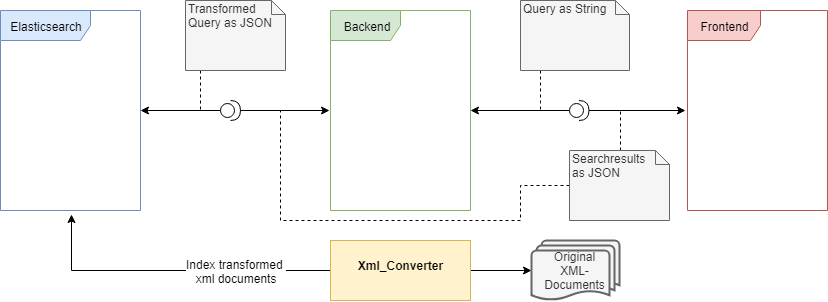
\includegraphics[width=\linewidth]{images/Architektur.png}
	\caption{Architektur des Systems}
\end{figure}

\subsection{Indizierungsprozess}

Die im Rahmen der Datenvorverarbeitung erstellten JSON-Dokumente werden mit \textit{Elasticsearch} mittels der bereitgestellten \texttt{bulk API} indiziert.
Die \texttt{bulk API} dient der Erhöhung der Indizierungsgeschwindigkeit.
Jede Seite einer Zeitung wird dabei in der Suchmaschine als eine JSON-Datei repräsentiert und enthält neben dem Veröffentlichungsdatum und weiteren Metadaten (Ausgabe, Seitenzahl, ...) die Texte der Zeitungsartikel.
Diese stellen den wichtigsten Bestandteil für die Indizierung dar, da in diesem relevante Terme enthalten sind, die von einem Nutzer gesucht werden können.
Wie jedoch bereits in den vorherigen Kapiteln dargelegt wurde, ist die Qualität der Terme durch eine Vielzahl von OCR-Scanartefakten beeinträchtigt.

\subsection{Suchprozess}

Ein Nutzer verfasst eine Suchanfrage, welche vom Client entgegengenommen und an das Backend weitergeleitet wird.
Das \textit{Flask}-Backend nimmt die Anfrage entgegen, konvertiert diese in eine \textit{Elasticsearch}-konforme Syntax und leitet diese an \textit{Elasticsearch} weiter.
\textit{Elasticsearch} transformiert diese Anfrage wiederum in das gleiche Format wie die bereits indizierten Dokumente.
Anschließend erfolgt der Vergleich der Suchterme mit den Termen der Dokumente im invertierten Index.
Auf Basis dieses Vergleichs wird ein Ranking der Dokumente nach absteigender Relevanz an das Backend zurückgegeben, welches dieses wiederum an das Frontend weiterleitet.
Im Frontend wird das Ranking der Dokumente dem Nutzer präsentiert.

\section{Vorstellung der Suchmaschine}

Nachdem der Indizierungs- und Suchprozess des Systems in Kapitel 4 erläutert wurde, erfolgt in diesem Kapitel die Vorstellung der Suchmaschine, insbesondere des User Interfaces.
Dabei wird zu 
Das User Interface besteht aus drei verschiedenen Sichen, die sich wie folgt darstellen:
	\begin{enumerate}
		\item Landing Page mit Eingabefeld für eine Suchanfrage
		\item Seite zur Auflistung der Suchergebnisse
		\item Seite zur Darstellung von Detailinformationen zu einer Zeitungsseite inklusive des zugehörigen Zeitungsscans  	
	\end{enumerate}
Bei der Beschreibung der Sichten erfolgt eine Erklärung der Prozesse die im System ablaufen.

\subsection{Landing Page}

Bei der \textit{Landing Page} handelt es sich, wie der Name schon sagt, um die Seite, die ein Nutzer sieht sobald dieser die Suchmaschine verwendet.
Auf dieser befindet sich neben einem thematisch passenden und ansprechenden Hintergrundbild ein Eingabefeld, in welcher die Nutzer eine Suchanfragen stellen können. 
Abbildung 1 zeigt die \textit{Landing Page} mit dem Eingabefeld für Suchanfragen.

\begin{figure}[h]
	
\includegraphics[width=\linewidth]{images/landing_page.png}
	\caption{Landing Page der Suchmaschine}
\end{figure}

\subsection{Auflistung der Suchergebnisse}

Nachdem ein Nutzer seine Suchanfrage in das Eingabefeld auf der \textit{Landing Page} eingegeben hat, wird diese an die \texttt{search}-Methode im Backend übergeben.
Wie bereits in Kapitel 3.2 beschrieben sucht diese in der Dokumentkollektion nach Zeitungsseiten, welche die Terme aus der Suchanfrage enthalten und gibt diese zurück. 
Die zurückgegebenen Zeitungen werden, nach ihrem Gewicht sortiert, in einer Liste von \textit{Cards} dargestellt.
Dabei wird eine Zeitungsseite von je einer \textit{Card} repräsentiert.
Diese enthalten neben einer Überschrift und dem Veröffentlichungsdatum ein kurzes Snippet, um dem Nutzer eine Vorschau auf die Artikel der Zeitungsseite zu bieten und diesen somit bei der Suche nach relevanten Ergebnissen zu unterstützen.
Weiterhin ist zur Gewährleistung der Übersichtlichkeit des User Interfaces eine \textit{Paginierung} implementiert.
Jede Seite enthält besitzt zehn Resultate. 
Abbildung 3 illustriert die Auflistung der Suchergebnisse für eine Suchanfrage nach der Partei \texttt{NSDAP}.

\begin{figure}[h]
	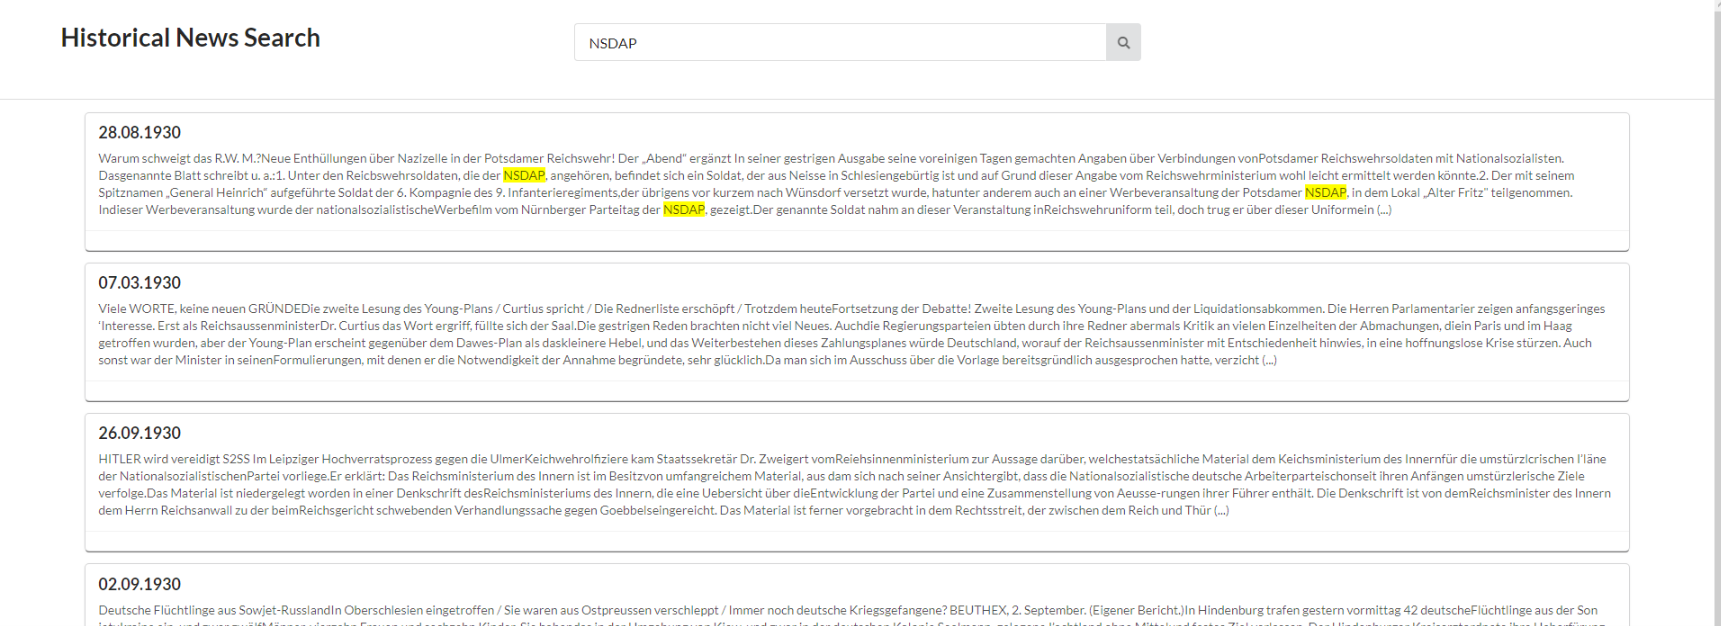
\includegraphics[width=\linewidth]{images/resultlist-view.png}
	\caption{Ergebnisliste zur Suchanfrage \texttt{NSDAP} mit Highlighting der Suchterme}
\end{figure}

\subsection{Detailansicht}

Klickt ein Nutzer auf eine der \textit{Cards} aus der Ergebnisliste, werden ihm sämtliche Artikel angezeigt, die auf der entsprechenden Zeitungsseite stehen sowie der Scan der Seite, sofern dieses vorhanden ist.
Abbildung 4 stellt die Detailansicht einer Zeitungsseite dar.
Darin ist die \textit{Split-View} zwischen Zeitungsscan und -text zu erkennen.


\begin{figure}[h]
	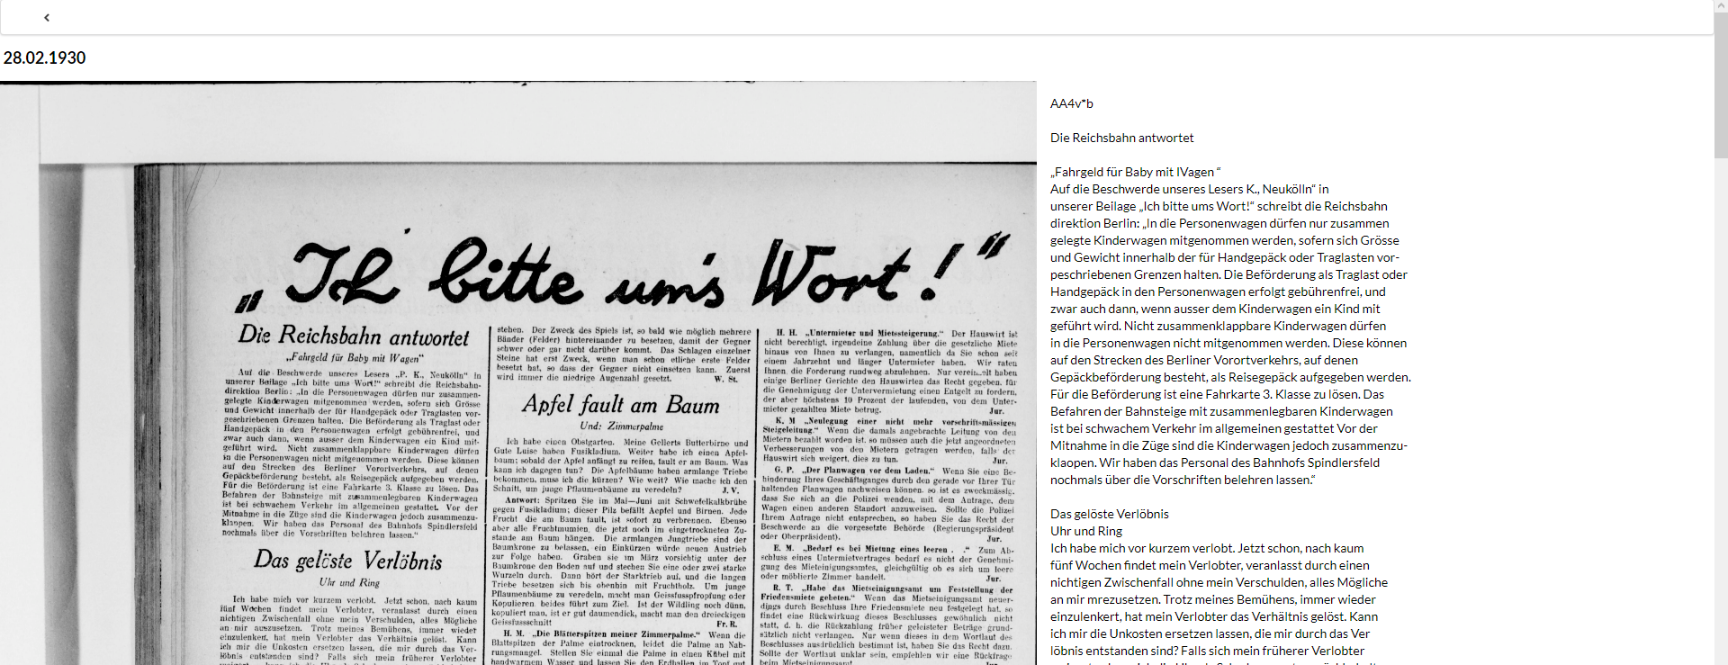
\includegraphics[width=\linewidth]{images/details-view.png}
	\caption{Detailansicht einer Zeitungsseite}
\end{figure}

\section{Evaluation}

Zur Effektivitätsmessung der \textit{Historical News Search} wird das Effektivitätsmaß \textit{Precision@k} sowie die daraus resultierenden Maße \textit{Average Precision} und \textit{Mean Average Precision} kalkuliert.
Der \textit{Precision}-Wert stellt den Anteil der relevanten Dokumente am Suchergebnis dar. 
Bei \textit{Precision@k} handelt es sich um den \textit{Precision}-Wert zu einem bestimmten \textit{Recall}-Level.
Grundlage für die Ermittlung, ob es sich bei einem Dokument um ein relevantes Dokument für eine gegebene Suchanfrage handelt, sind die von den Gruppenmitgliedern bereitgestellten Relevanzurteile.
Die Relevanzurteile definieren, ob ein Dokument für ein Informationsbedürfnis relevant ist und bewegen sich im binären Spektrum zwischen \textit{Relevant} und \textit{Nicht relevant}.
Ein Informationsbedürfnis wird in Form eines \textit{Topics} modelliert.
Ein \textit{Topic} besteht aus drei Elementen, welche in Tabelle 2 exemplarisch für ein gewähltes \textit{Topic} gezeigt werden. 

\begin{table}[h]
	\centering
	\begin{tabularx}{\textwidth}{|c|p{9.55cm}|}
		\hline 
		& \textbf{Topic} \\ 
		\hline 
		\textbf{Suchanfrage} & Theodore Roosevelt \\ 
		\hline 
		\textbf{Beschreibung} & Wie berichtete die deutsche Presse über Theodore Roosevelt zu seiner Zeit als Präsident der Vereinigten Staaten von Amerika zwischen 1901 und 1908? \\ 
		\hline 
		\textbf{Narrativ} & Relevante Dokumente enthalten Zeitungsartikel zu Theodore Roosevelt, dem 26. Präsidenten der Vereinigten Staaten. Relevante Details enthalten Informationen von Theodore Roosevelts politischen Aktivitäten und der Bewertung und Einordnung dieser in der deutschen Presse. \\ 
		\hline 
	\end{tabularx}
\caption{Modellierung eines Topics}
\end{table}

Im Folgenden wird kurz die Vorgehensweise bei der Evaluation vorgestellt und erklärt, welche Schritte zur Verbesserung der Effektivität der Suchmaschine unternommen wurden.
Abschließend werden die erzielten Resultate dargestellt und eingeordnet.

\subsection{Methodik}

Die Evaluation durchläuft zwei Iterationen.
In den beiden Evaluationsiterationen werden für die rund 40 definierten Topics die jeweiligen \textit{Average Precision}-Werte berechnet. 
Grundlage für die Berechnung stellen die bereitgestellten binären Relevanzurteile dar.
Aus den \textit{Average Precision}-Werten wird wiederum das arithmetische Mittel kalkuliert, um die \textit{Mean Average Precision} zu erhalten.
Diese stellt das bedeutenste \textit{Effektivitätsmaß} für die Evaluation des Systems dar, da dieses den Vergleich zweier Systeme auf ein Maß herunterbricht.

In der ersten Iteration erfolgt die initiale Evaluation der Suchmaschine mit sämtlichen standardmäßigen Einstellungen von \textit{Elasticsearch}.
Anschließend erfolgt das Refinement des Systems, bestehend aus der Anpassung von Parametern sowie der Implementierung zusätzlicher Funktionen. 
Die Maßnahmen, die im Refinement zur Steigerung der Effektivität des Systems unternommen werden sind folgenden Kapitel näher beschrieben. 
Nach Abschluss des Refinements erfolgt die zweite Evaluationsiteration mit abschließendem Vergleich der beiden Systeme. 

\subsection{Refinement}

Die Optimierung des Retrieval-Prozesses erfolgt durch mehrere Maßnahmen, welche im Folgenden näher erläutert werden.
Während der durchgeführten, ersten Evaluationsiteration ist festzustellen, dass Stoppwörter zu gleichem Maße in die Berechnung des Scores eines Dokumentes eingehen, wie die anderen Terme.
Dadurch verlieren andere, wichtigere Terme an Gewicht bei der Erstellung des Scores, was zu einer schlechteren Platzierung von relevanten Dokumenten führt.
Daher bietet sich die Optimierungsmethode des \textit{Stoppings} an, um eine Verbesserung der Retrievalperformanz zu erreichen.

Unter \textbf{Stopping} versteht man das Entfernen von Stoppwörtern aus der Menge der Indexterme.
Stoppwörter bezeichnen Wörter, welche häufig anzutreffen sind und keine Relevanz für die Erfassung des Dokumenteninhalts besitzen.
\textit{Elasticsearch} bietet die Möglichkeit vordefinierte sowie selbsterstellte Stopwortlisten zu verwenden.
Zur Implementierung des \textit{Stoppings} wird die vorgefertigte Stoppwortliste für die deutsche Sprache sowie zusätzlich eine eigene Stoppwortliste mit ergänzenden Wörtern verwendet. 

Zur gezielten Suche nach bestimmten Attributen wird außerdem eine eigene \textbf{Query Syntax} eingebaut. 
Bei den Attributen handelt es sich um die in Listing 1 gezeigten Attribute der JSON-Dokumentrepräsentationen.
Ein Nutzer ist beispielsweise in der Lage durch Eingabe der Suchanfrage \texttt{year:1930 month:01} nach Zeitungsartikeln vom Januar 1930 zu suchen.
Durch diese Funktion ist eine gezieltere Suche insbesondere für erfahrene Nutzer möglich.

Zur Verbesserung der Nutzererfahrung wird ein \textbf{Highlighting} der in der Suchanfrage enthaltenen Terme implementiert.
Weiterhin werden dem Nutzer während der Erstellung der Suchanfrage \textbf{Vorschläge zur Vervollständigung} angeboten.
Diese Funktionen verhindern orthografische Fehler bei der Eingabe und gewährleisten eine schnellere Erkennung von relevanten Dokumenten durch den Nutzer.

\subsection{Resultat}

In der ersten Evaluationsiteration wurde eine \textit{Mean Average Precision} von 0,39 erzielt.
Trotz Implementierung der im vorherigen Kapitel vorgestellten Optimierungen wurde auch nach einer zweiten Evaluationsiteration eine \textit{Mean Average Precision} von 0,39 erzielt.
Folglich ist mit den verwendeten Optimierungsansätzen keine Verbesserung der Retrievalperformanz eingetreten.
Einzig die Nutzererfahrung konnte durch die vorgestellten Optimierungsansätze verbessert werden, was sich jedoch nicht quantitativ belegen lässt.

\section{Zusammenfassung und Ausblick}

Die in diesem Bericht betrachtete Suchmaschine mit dem Titel \textit{Historical News Search} ermöglicht seinen Nutzern eine benutzerfreundliche Möglichkeit nach historischen Zeitungsartikeln der \textit{Berliner Volkszeitung} zu suchen.
Das vorgestellte Web-Interface bietet eine benutzerfreundliche Möglichkeit der Nutzerinteraktion sowie eine übersichtliche Darstellung der Resultate.
Durch verschiedene Optimierungsansätze (Stopping, eigene Query Syntax, ...) und unter Verwendung der bereitgestellten Indizierungs- und Suchfunktion der Open Source Suchmaschine \textit{Elasticsearch} konnte eine \textit{Mean Average Precision} von XXX erzielt werden.

Der verwendete Datensatz der \textit{Staatsbibliothek zu Berlin} enthält eine Vielzahl von OCR-Scanartefakten, welche vor allem auf die altdeutsche Schrift zurückzuführen sind.
Diese schränken die Suchmaschine stark bei der Suche nach relevanten Dokumenten ein. 
Zur Weiterentwicklung der Suchmaschine wäre es demnach sinnvoll dieses Problem vorrangig zu adressieren und Anstrengungen zu unternehmen die Scanartefakte möglichst vollständig zu eliminieren.
Dadurch würde sich die Performanz der Suchmaschine und folglich auch die Nutzererfahrung erheblich verbessern.

Eine weitere Verbesserung der Suchmaschine, insbesondere in Bezug auf die Nutzerfreundlichkeit, würde die Extraktion und Darstellung der einzelnen Artikel einer Seite mit sich bringen.
Auf diese Weise würde der Nutzer direkt zu dem von ihm gewünschten relevanten Artikel gelangen, ohne die irrelevanten Artikel einer Seite betrachten zu müssen.  

Interessant ist ebenfalls die Änderung des verwendeten Retrievalmodells und der Einfluss dessen auf die Performanz des Systems.
Dieser Einfluss kann ebenfalls in einer weiteren Entwicklung genauer evaluiert werden, indem verschiedene andere Retrievalmodelle eingesetzt und verglichen werden.
In diesem Zusammenhang ist es auch möglich, das Spektrum der Relevanzurteile zu erweitern, um eine stärkere Differenzierung der Relevanz von Dokumenten zu gegebenen Suchanfragen während des Suchprozesses nutzen zu können.

% ----------------------------------------------------------------------------

% \newpage
% \begin{footnotesize}

% IF YOU DO NOT USE BIBTEX, USE THE FOLLOWING SAMPLE SCHEME FOR THE REFERENCES
% ----------------------------------------------------------------------------

% \begin{thebibliography}{99}

% For articles
%\bibitem{1}David Caswell, Konstantin Dörr, "Automated Journalism 2.0: Event-driven naratives", \emph{Journalism Practice}, 09.05.2017.

%\bibitem{2}Andreas Graefe, "Guide to Automated Journalism", \emph{Columbia University Academic Commons}, 07.01.2016.

%\bibitem{3}L. Leppänen, M. Munezero, M. Granroth-Wilding, H. Toivonen, "Data-Driven News Generation for Automated Journalism", \emph{University of Helsinki}, 2017

%\bibitem{4}Retresco GmbH, ``Retresco - Textgenerierung'', \emph{\\https://www.retresco.de/textgenerierung/}, zuletzt abgerufen 01.07.2018

%\bibitem{5}DFL Deutsche Fußball Liga GmbH, ``Schalke 04 krönt Saison mit Heimsieg - Eintracht Frankfurt verpasst vorerst Europa'', \emph{https://www.bundesliga.com/de/bundesliga/news/fc-schalke-04-eintracht-frankfurt-34-spieltag-spielbericht.jsp}, zuletzt abgerufen 01.07.2018

%\bibitem{6}Statistik zum Spiel FC Bayern München - Vfb Stuttgart auf Bundesliga.de, \\
%\emph{https://www.bundesliga.com/de/bundesliga/spieltag/2017-2018/34-fc\_bayern\_muenchen-vfb\_stuttgart.jsp?statistics}, zuletzt abgerufen 24.08.2018

% \end{thebibliography}
%
%\section{Abbildungsverzeichnis}
%


% IF YOU USE BIBTEX,
% - DELETE THE TEXT BETWEEN THE TWO ABOVE DASHED LINES
% - UNCOMMENT THE NEXT TWO LINES AND REPLACE 'Name_Of_Your_BibFile'

%\bibliographystyle{unsrt}
%\bibliography{Name_Of_Your_BibFile}

% \end{footnotesize}

\end{document}